
    \usetikzlibrary{shapes.callouts}
    \tikzset{
      level/.style   = { ultra thick, blue },
      connect/.style = { dashed, red },
      notice/.style  = { draw, rectangle callout, callout relative pointer={#1} },
      label/.style   = { text width=2cm }
    }
    
    \scalebox{0.75}{
    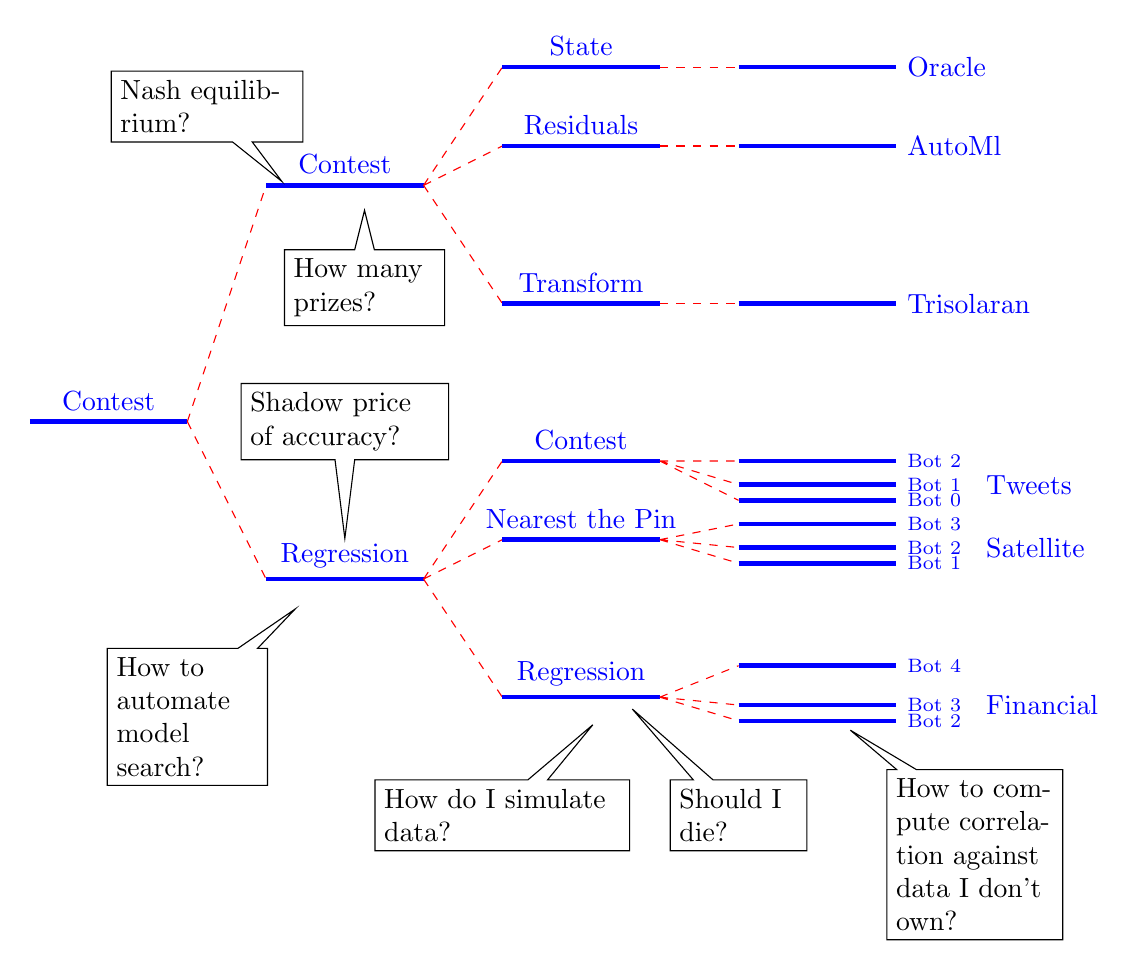
\begin{tikzpicture}
       % Draw all levels
      \draw[level] (0,0) -- node[above] {Contest}  (2,0);
    
      \draw[connect] (2,0)  -- (3,-2) (2,0) -- (3,3);
      \draw[level]   (3,3)  -- node[above] {Contest} node[below] {} (5,3);
      \draw[level]   (3,-2) -- node[above] {Regression} node[below] {} (5,-2);
    
      \draw[connect] (5,3)    -- (6,4.5) (5,3) -- (6,3.5) (5,3) -- (6,1.5);
      \draw[connect] (5,-2)   -- (6,-0.5) (5,-2) -- (6,-1.5) (5,-2) -- (6,-3.5);
      \draw[level]   (6,4.5)  -- node[above] {State} (8,4.5);
      \draw[level]   (6,3.5)  -- node[above] {Residuals} (8,3.5);
      \draw[level]   (6,1.5)  -- node[above] {Transform} (8,1.5);
      \draw[level]   (6,-0.5) -- node[above] {Contest} (8,-0.5);
      \draw[level]   (6,-1.5) -- node[above] {Nearest the Pin} (8,-1.5);
      \draw[level]   (6,-3.5) -- node[above] {Regression} (8,-3.5);
    
      \draw[connect] (8,4.5) -- (9,4.5) (8,3.5) -- (9,3.5) (8,1.5) -- (9,1.5);
      \draw[level]   (9,4.5) -- (11,4.5) node[right] {Oracle};
      \draw[level]   (9,3.5) -- (11,3.5) node[right] {AutoMl};
      \draw[level]   (9,1.5) -- (11,1.5) node[right] {Trisolaran};
    
      \draw[connect] (8,-0.5) -- (9,-0.5) (8,-0.5) -- (9,-0.8) (8,-0.5) -- (9,-1)
                     (8,-1.5) -- (9,-1.6) (8,-1.5) -- (9,-1.8) (8,-1.5) -- (9,-1.3)
                     (8,-3.5) -- (9,-3.8) (8,-3.5) -- (9,-3.6) (8,-3.5) -- (9,-3.1);
      \foreach \i/\j in {2/-0.5, 1/-0.8, 0/-1} {
        \draw[level] (9,\j) -- (11,\j) node[right] {\scriptsize Bot $\i$};
      }
      \node[level, right] at (12,-0.8) {Tweets};
      \foreach \i/\j in {3/-1.3, 2/-1.6, 1/-1.8} {
        \draw[level] (9,\j) -- (11,\j) node[right] {\scriptsize Bot $\i$};
      }
      \node[level, right] at (12,-1.6) {Satellite};
      \foreach \i/\j in {4/-3.1, 3/-3.6, 2/-3.8} {
        \draw[level] (9,\j) -- (11,\j) node[right] {\scriptsize Bot $\i$};
      }
      \node[level, right] at (12,-3.6) {Financial};
    
      % Draw labels
     % \node[label] at (4,5.5)  {Depth 1};
     % \node[label] at (7,5.5)  {Depth 2};
     % \node[label] at (10,5.5) {Depth 3};
    
      % Draw annotations
       \node[notice={(0,0.5)}, text width=1.8cm] at (4.25,1.7) {How many prizes?};
       \node[notice={(0.5,-0.5)}, text width=2.2cm] at (2.25,4) {Nash equilibrium?};
     
      \node[notice={(0.5,0.5)}, text width=1.8cm] at (2,-3.75) {How to automate model search?};
      \node[notice={(0,-1)}, text width=2.4cm] at (4,0) {Shadow price of accuracy?} ;
      \node[notice={(0.7,0.7)}, text width=3cm] at (6,-5)
        {How do I simulate data?};
      \node[notice={(-0.9,0.9)}, text width=1.5cm] at (9,-5) {Should I die?};
      \node[notice={(-0.5,0.5)}, text width=2cm] at (12,-5.5) {How to compute correlation against data I don't own?};
    \end{tikzpicture}
    }
